% Task 4: X25519. Values from Task4/ecdh.py (the private keys of RFC 7748, section 6.1).
% CHECKED (python3, Task4/solution/ecdh.py): both secrets are equal; the public keys, the secret and the key
%   are the results of the task, so the figure shows them as unknown
\documentclass[12pt,tikz,border=6pt]{standalone}
% Shared preamble of the task figures of Lecture 5 (based on Lecture2/task-figures/common.tex).
% The roles take the colours of the elliptic-curves simulator (CryptographySimulators/elliptic-curves),
% so that the README figures and the simulator look the same:
%   secret (number or point): amber, public point: violet, Alice: blue, Bob: green,
%   Eve: red, ciphertext: brown, message: grey, a change or the unknown: orange.
\usepackage{lmodern}
\usepackage[T1]{fontenc}
\renewcommand{\familydefault}{\sfdefault}
\usepackage{amsmath,amssymb}
\usepackage{xcolor}
\usepackage{fontawesome5}
\usetikzlibrary{arrows.meta, calc, positioning, fit, decorations.pathreplacing, backgrounds}

% ---------- template and neutral ----------
\definecolor{DeepBlue}{HTML}{283593}
\definecolor{AccentOrange}{HTML}{EB5A14}
\definecolor{nInk}{HTML}{37474F}
\definecolor{nLine}{HTML}{90A4AE}
\definecolor{nLight}{HTML}{CFD8DC}
\definecolor{nFill}{HTML}{ECEFF1}
\definecolor{aExec}{HTML}{43A047}
\definecolor{aWrite}{HTML}{E53935}

% ---------- roles (the colours of the elliptic-curves simulator) ----------
\definecolor{rPriv}{HTML}{E2A60E}  \definecolor{rPrivBg}{HTML}{FDF3DC}  \definecolor{rPrivText}{HTML}{9A6B00}
\definecolor{rPub}{HTML}{8A5CD8}   \definecolor{rPubBg}{HTML}{F1EAFD}   \definecolor{rPubText}{HTML}{6A3FB8}
\definecolor{rAli}{HTML}{2F6FDB}   \definecolor{rAliBg}{HTML}{E5EDFB}
\definecolor{rBob}{HTML}{2FA84F}   \definecolor{rBobBg}{HTML}{E3F4E8}   \definecolor{rBobText}{HTML}{1E7E4F}
\definecolor{rEve}{HTML}{E5484D}   \definecolor{rEveBg}{HTML}{FDE9E9}
\definecolor{rCip}{HTML}{A8642A}   \definecolor{rCipBg}{HTML}{F7ECE0}
\definecolor{rMsg}{HTML}{BCC4CC}   \definecolor{rMsgBg}{HTML}{EEF1F4}
\definecolor{rChg}{HTML}{D9621C}   \definecolor{rChgBg}{HTML}{FCE8DA}

\tikzset{
  hw/.style={draw=nLine, thick, fill=nFill, text=nInk, rounded corners=3pt, align=center, inner sep=4pt},
  hwmain/.style={draw=nInk, thick, fill=nInk, text=white, rounded corners=3pt, align=center, inner sep=4pt},
  role/.style={draw=#1, thick, fill=#1Bg, text=nInk, rounded corners=3pt, align=center, inner sep=5pt},
  unk/.style={draw=rChg, thick, dashed, fill=white, text=rChg, rounded corners=3pt, align=center, inner sep=5pt,
    font=\bfseries},
  data/.style={-{Stealth}, very thick, nInk},
  note/.style={font=\small, text=nInk},
  person/.style={circle, fill=#1, draw=#1, text=white, minimum size=1.1cm, font=\Large, inner sep=0pt},
}
\newcommand{\personnode}[4]{%
  \node[person=#3] (#1) at (#2) {\faUser};
  \node[font=\small\bfseries, text=#3, below=0.06cm of #1] (#1lbl) {#4};}
\newcommand{\cogbox}[4]{%
  \node[hwmain, minimum width=#4, minimum height=1.1cm] (#1) at (#2) {};
  \node[text=white, font=\large, anchor=west] at ([xshift=0.2cm]#1.west) {\faCogs};
  \node[text=white, font=\small\bfseries] at ([xshift=0.3cm]#1.center) {#3};}

% ---------- the toy curve y^2 = x^3 + 2x + 2 mod 17 (as on the slides) ----------
% CHECKED: python3, all (x, y) with 0 <= x, y < 17 and y^2 = x^3 + 2x + 2 mod 17: these 18 points
\newcommand{\curvepts}{0/6,0/11,3/1,3/16,5/1,5/16,6/3,6/14,7/6,7/11,9/1,9/16,10/6,10/11,13/7,13/10,16/4,16/13}
% the grid of dots, in grid coordinates (1 unit = one step of x or y); draw it inside a scope
\newcommand{\gridbody}{%
  \foreach \x in {0,...,16} \foreach \y in {0,...,16} \fill[nLight] (\x,\y) circle (1.1pt);
  \draw[nLine, thick] (-0.7,-0.7) -- (16.7,-0.7);
  \draw[nLine, thick] (-0.7,-0.7) -- (-0.7,16.7);
  \foreach \v in {0,...,16} {
    \node[font=\tiny, text=gray, anchor=north] at (\v,-0.75) {\v};
    \node[font=\tiny, text=gray, anchor=east] at (-0.75,\v) {\v};
  }
  \node[font=\scriptsize, text=nInk, anchor=west] at (16.8,-0.7) {$x$};
  \node[font=\scriptsize, text=nInk, anchor=south] at (-0.7,16.8) {$y$};
  \foreach \x/\y in \curvepts \fill[nInk] (\x,\y) circle (3pt);}
% mark a point of the grid: \gmark[colour]{x,y}{label}{where the label goes}
\newcommand{\gmark}[4][rPub]{%
  \node[circle, draw=#1, line width=1.2pt, fill=#1, minimum size=9pt, inner sep=0pt] at (#2) {};
  \node[font=\scriptsize\bfseries, text=#1, #4, inner sep=1pt, outer sep=3pt, fill=white, fill opacity=0.85,
    text opacity=1, rounded corners=1pt] at (#2) {#3};}

\begin{document}
\pagecolor{white}
\begin{tikzpicture}[>=Stealth]
  \personnode{alice}{0,0}{rAli}{Alice}
  \personnode{bob}{12,0}{rBob}{Bob}
  % private keys
  \node[role=rPriv, font=\scriptsize\ttfamily, anchor=north, text width=3.4cm, align=left] (pa) at (0,-1.25)
    {\textbf{\normalfont\small\faKey\ private (32 bytes)}\\ 77076d0a7318a57d\ldots\\ \ldots b177fba51db92c2a};
  \node[role=rPriv, font=\scriptsize\ttfamily, anchor=north, text width=3.4cm, align=left] (pb) at (12,-1.25)
    {\textbf{\normalfont\small\faKey\ private (32 bytes)}\\ 5dab087e624a8a4b\ldots\\ \ldots 1c2f8b27ff88e0eb};
  % public keys
  \node[unk, font=\small\bfseries, draw=rPub, text=rPubText, fill=rPubBg] (qa) at (3.6,0.2) {public A = ?};
  \node[unk, font=\small\bfseries, draw=rPub, text=rPubText, fill=rPubBg] (qb) at (8.4,0.2) {public B = ?};
  \draw[data] (alice) -- node[above, font=\scriptsize\ttfamily, text=nInk] {public\_key} (qa);
  \draw[data] (bob) -- node[above, font=\scriptsize\ttfamily, text=nInk] {public\_key} (qb);
  \draw[data, rPub] (qa.north) to[bend left=25] node[above, font=\scriptsize, text=nInk, pos=0.5] {to Bob} ([xshift=0.6cm]qb.north);
  \draw[data, rPub] (qb.south) to[bend left=25] node[below, font=\scriptsize, text=nInk, pos=0.5] {to Alice} ([xshift=-0.6cm]qa.south);
  % Eve
  \node[person=rEve, minimum size=0.9cm, font=\normalsize] (eve) at (6,2.6) {\faUserSecret};
  \node[font=\scriptsize\bfseries, text=rEve, anchor=west] at (6.5,2.55) {Eve sees A and B};
  \draw[rEve, thick, dashed] (eve.south) -- (6,1.55);
  % shared secrets
  \node[unk, font=\small\bfseries, draw=rPriv, text=rPrivText, fill=rPrivBg, anchor=north] (sa) at (3.9,-2.3) {secret = ?};
  \node[unk, font=\small\bfseries, draw=rPriv, text=rPrivText, fill=rPrivBg, anchor=north] (sb) at (8.1,-2.3) {secret = ?};
  \draw[data] (pa.east |- sa) -- (sa.west);
  \node[font=\scriptsize\ttfamily, text=nInk, anchor=south] at (sa.north) {x25519(private, B)};
  \draw[data] (pb.west |- sb) -- (sb.east);
  \node[font=\scriptsize\ttfamily, text=nInk, anchor=south] at (sb.north) {x25519(private, A)};
  \node[font=\large\bfseries, text=rChg] (eq) at (6,-2.6) {$=$ ?};
  % HKDF
  \cogbox{kdf}{6,-4.0}{hkdf}{2.6cm}
  \draw[data] (sa.south) |- (kdf.west);
  \node[font=\scriptsize\ttfamily, text=gray, anchor=north] at (kdf.south) {info = b"lecture 5 chat key"};
  \node[unk, font=\small\bfseries, draw=rPriv, text=rPrivText, fill=rPrivBg, anchor=west] (key) at (8.2,-4.0) {ChaCha20 key, 32 bytes = ?};
  \draw[data] (kdf.east) -- (key.west);
\end{tikzpicture}
\end{document}
